\section{Theory}

	\subsection{Interference}

	Albert Michelson created an Interferometer, which was used to detect luminiferous ether in the late 19th century. The experiment uses it to measure the wavelength of light and is based on the interference of light. A beam splitter divides a source beam into two parts which form an intereference pattern on a screen upon getting reflected back from 2 mirrors. The setup is shown in \hyperref[fig:1]{Figure 1}.

		\begin{figure}[H]
			\centering
			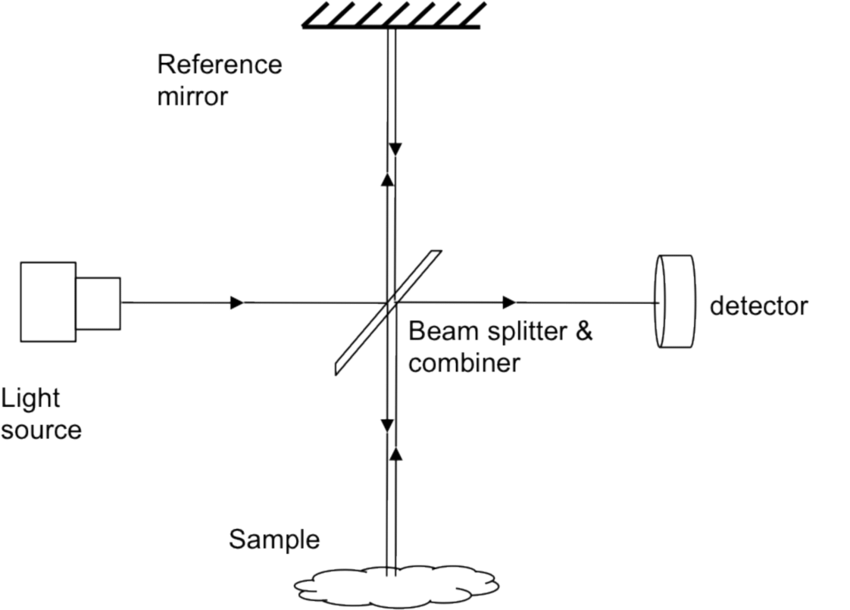
\includegraphics[width=0.4\textwidth]{images/michelson_interferometer.png}
			\caption{Michelson Interferometer}
			\label{fig:1}
		\end{figure}

		The interference can be of two types:

		\begin{enumerate}
			\item \textbf{Constructive interference:} When the path difference is a multiple of the wavelength. This is the case when the path difference is a multiple of the wavelength, i.e. $\Delta d = n\lambda$.
			\item \textbf{Destructive interference:} When the path difference is not a multiple of the wavelength. This is the case when the path difference is not a multiple of the wavelength, i.e. $\Delta d = (n + \frac{1}{2})\lambda$.
		\end{enumerate}

	\subsection{Types of Fringes}
		
		The fringes observed are of the following types depending on the orientation of the mirrors:

		\begin{itemize}
			\item \textbf{Concentric circular fringes (fringes of equal inclination):} This occurs when the image of mirror $M_2$ as seen through the beam splitter is exactly parallel to the mirror $M_1$ or simply when $M_2$ is perpendicular to $M_1$. Since the width of the air film between the image and M1 is constant, the fringes are formed depending on the inclination of the reflected and incident rays. If the angle is say, $\theta$, then the ray reflecting from the further away mirror will travel a extra distance of $2d$ cos $\theta$ as shown in figure below.
			\begin{figure}[H]
				\centering
				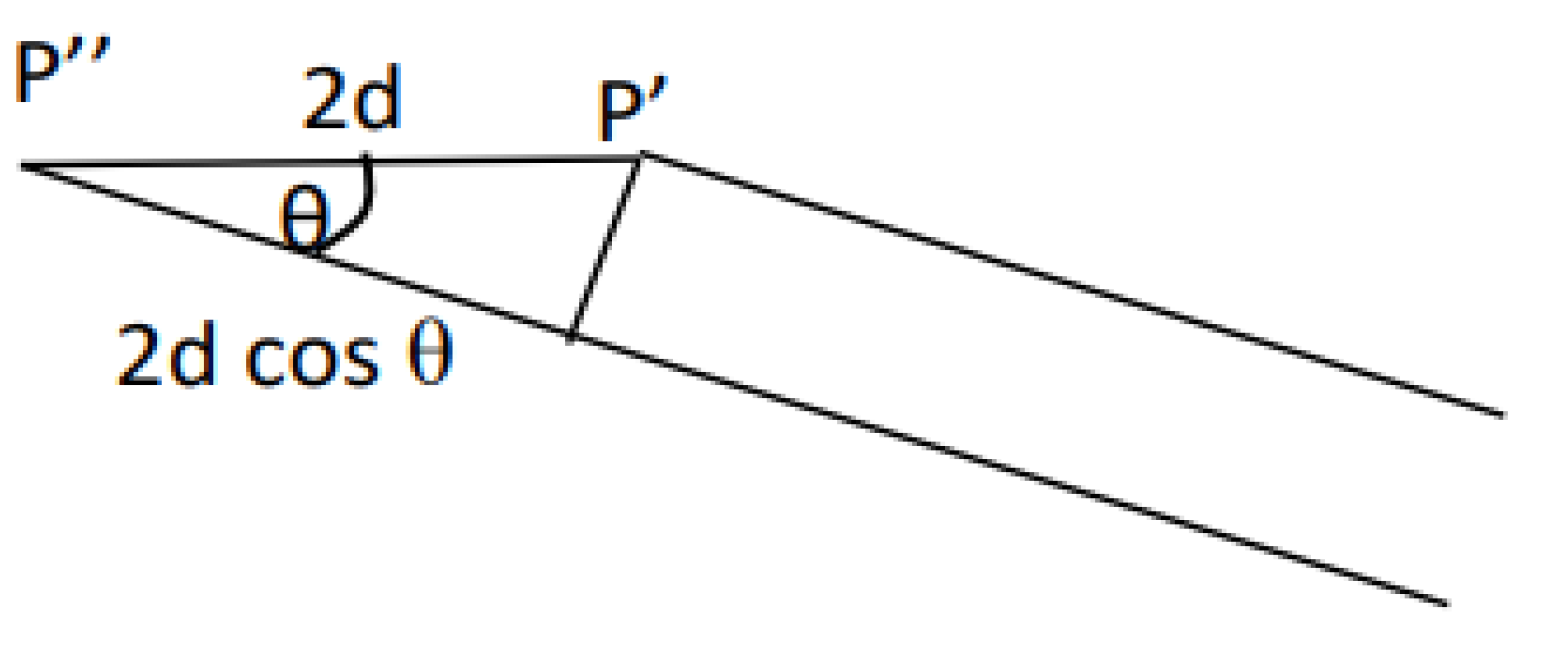
\includegraphics[width=0.25\textwidth]{images/1.png}
			\end{figure}
			\begin{figure}[H]
				\centering
				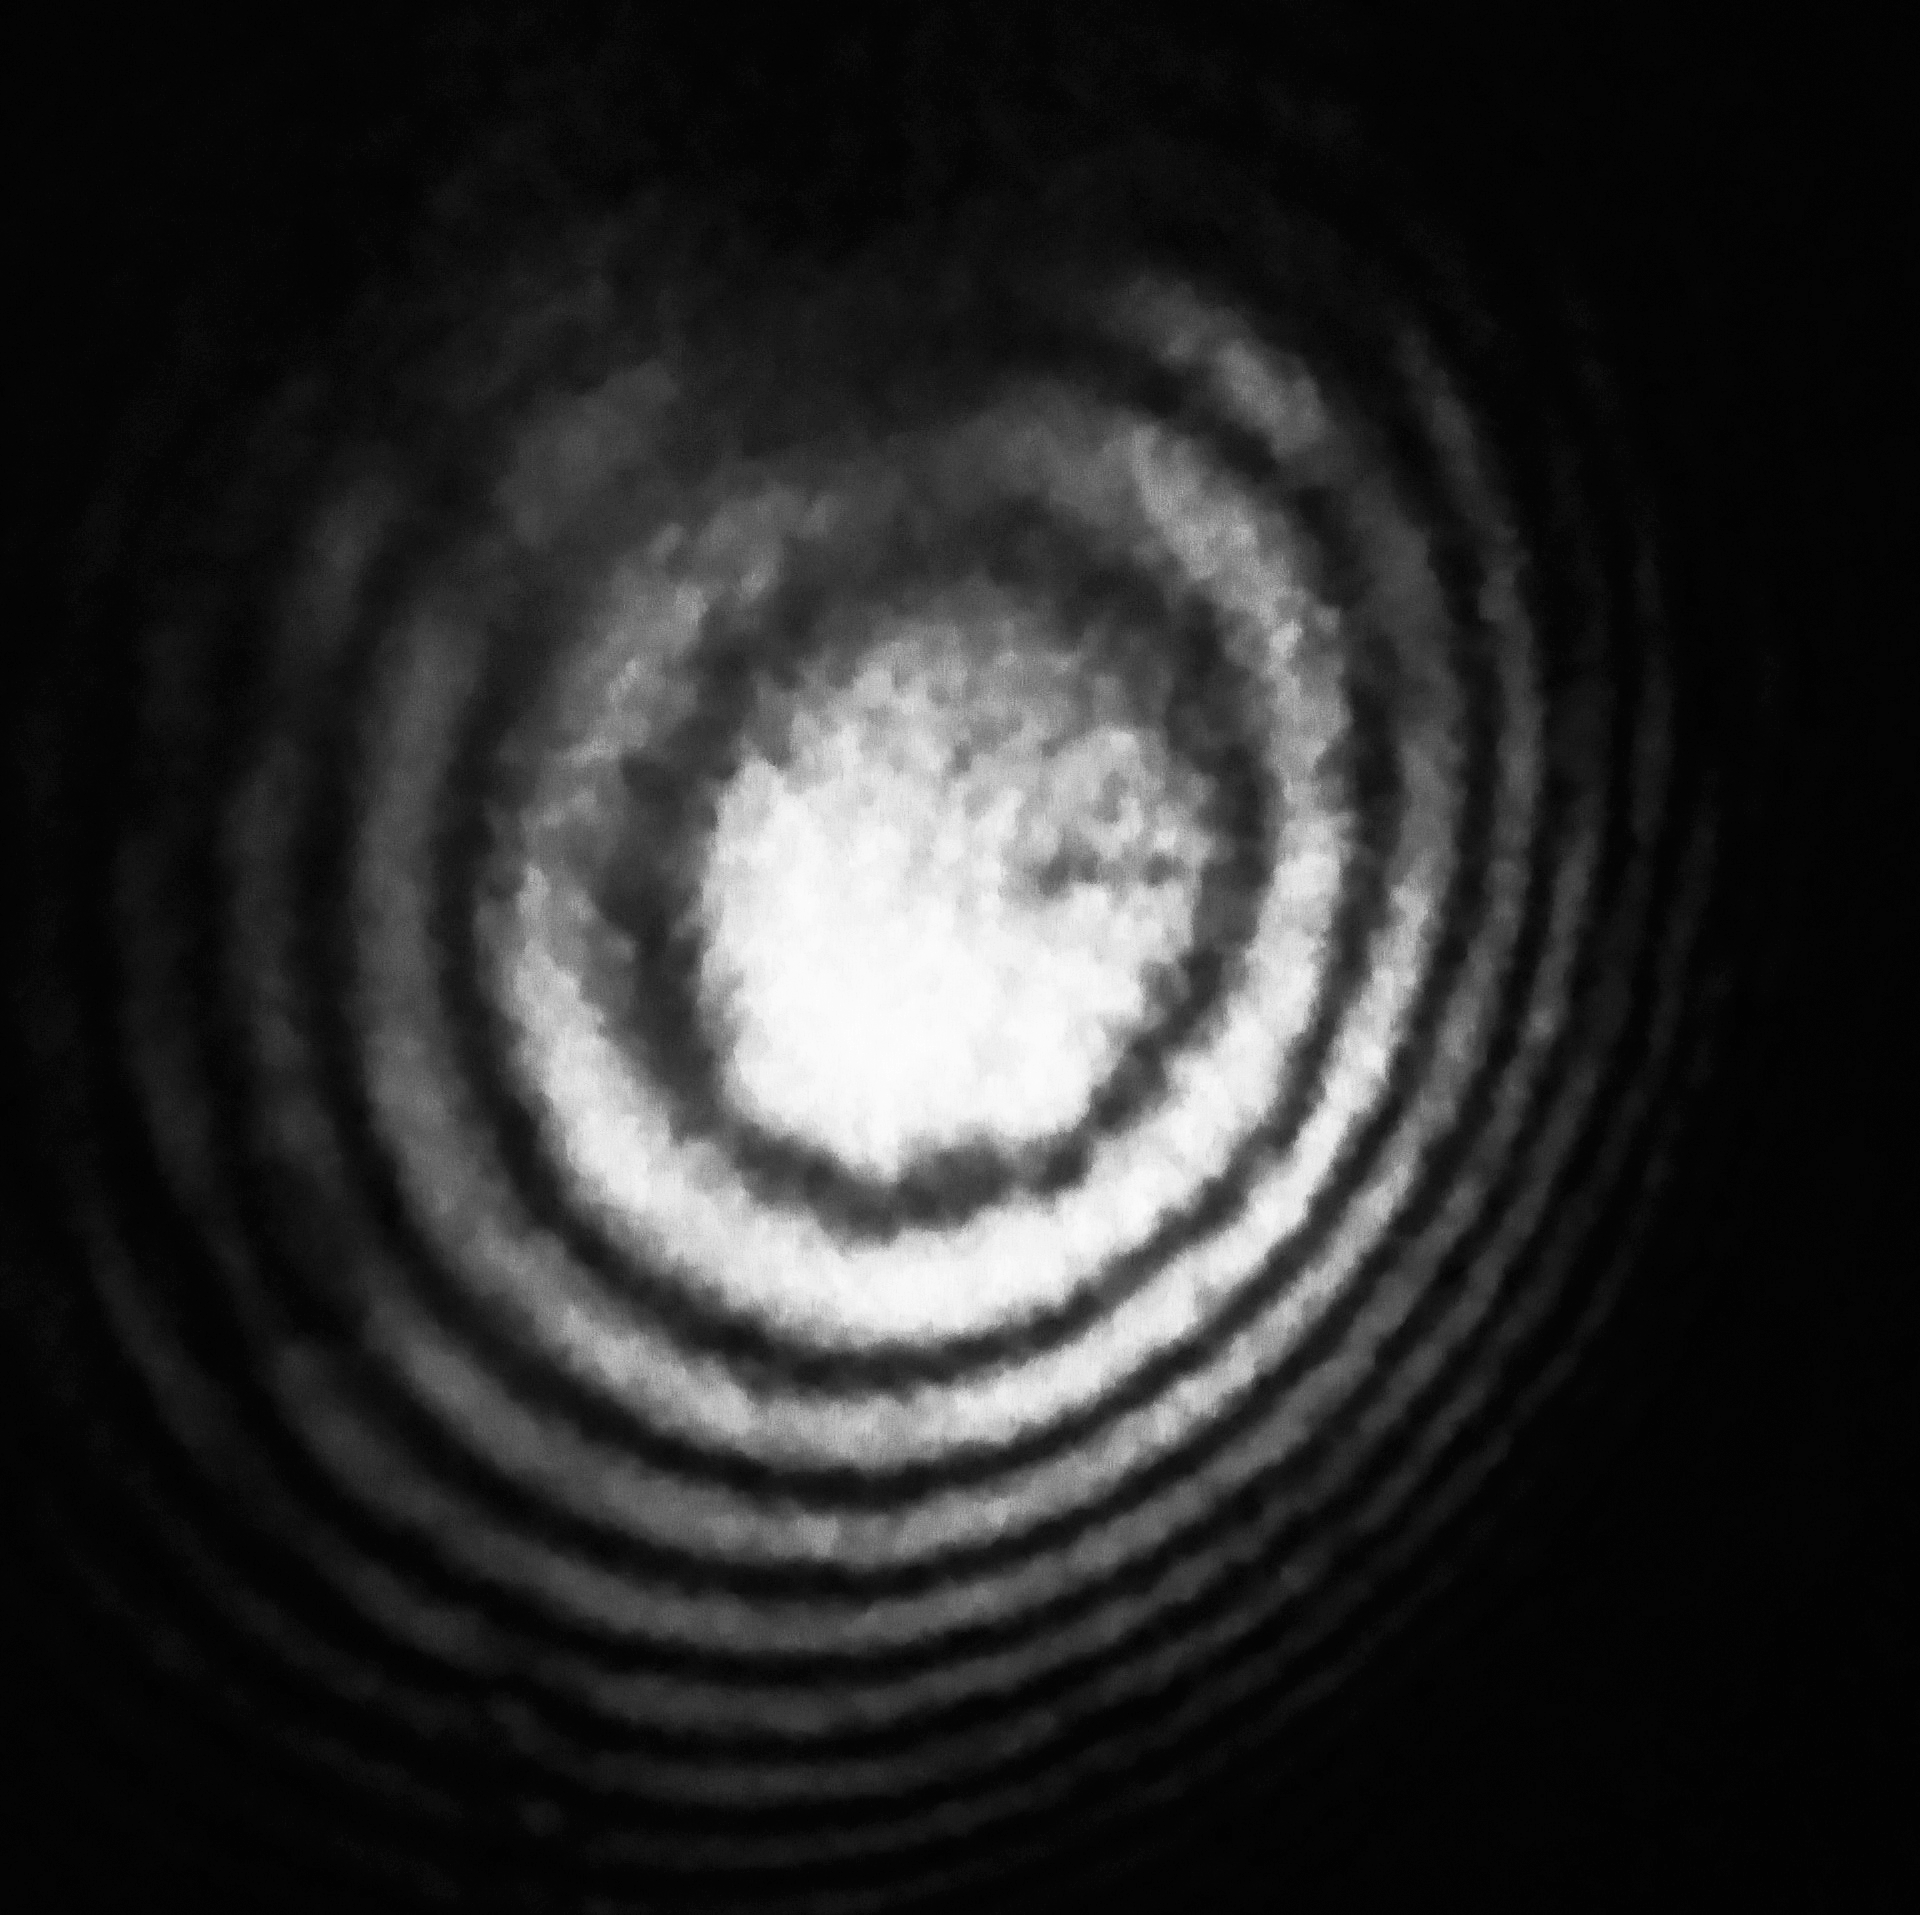
\includegraphics[width=0.25\textwidth]{images/circular_g.jpg}
				\caption{Circular fringes for He-Ne Lazer}
			\end{figure}
			Therefore bands will be formed for the same inclination of light rays which corresponds to circular fringes. In the experiment we will deal with circular fringes for the two light source. As we change the path difference between the mirror from $d (2d = n\lambda)$, say $N$ fringes appear or disappear near the centre (that is inclination $\theta = 0$. This implies:
			$$2(d+\Delta d) = (n+N)\lambda$$
			\begin{equation}
				2\Delta d = N\lambda
				\label{eq:1}
			\end{equation}
			It is because each fringe corresponded to a particular multiple of wavelength. The images of the circular fringes formed in the experiment for He-Ne laser are shown below.


			\item \textbf{Curved fringes (fringes of equal thickness):} This occurs when the mirror M1 and M2 (or its image as in previous point) are inclined at an angle such that the width between the two forms a wedge. Hence the fringes will be common for the path difference of a particular thickness leading to curved (hyperbolic) to straight line fringes as shown in figure below.
			\begin{figure}[H]
				\centering
				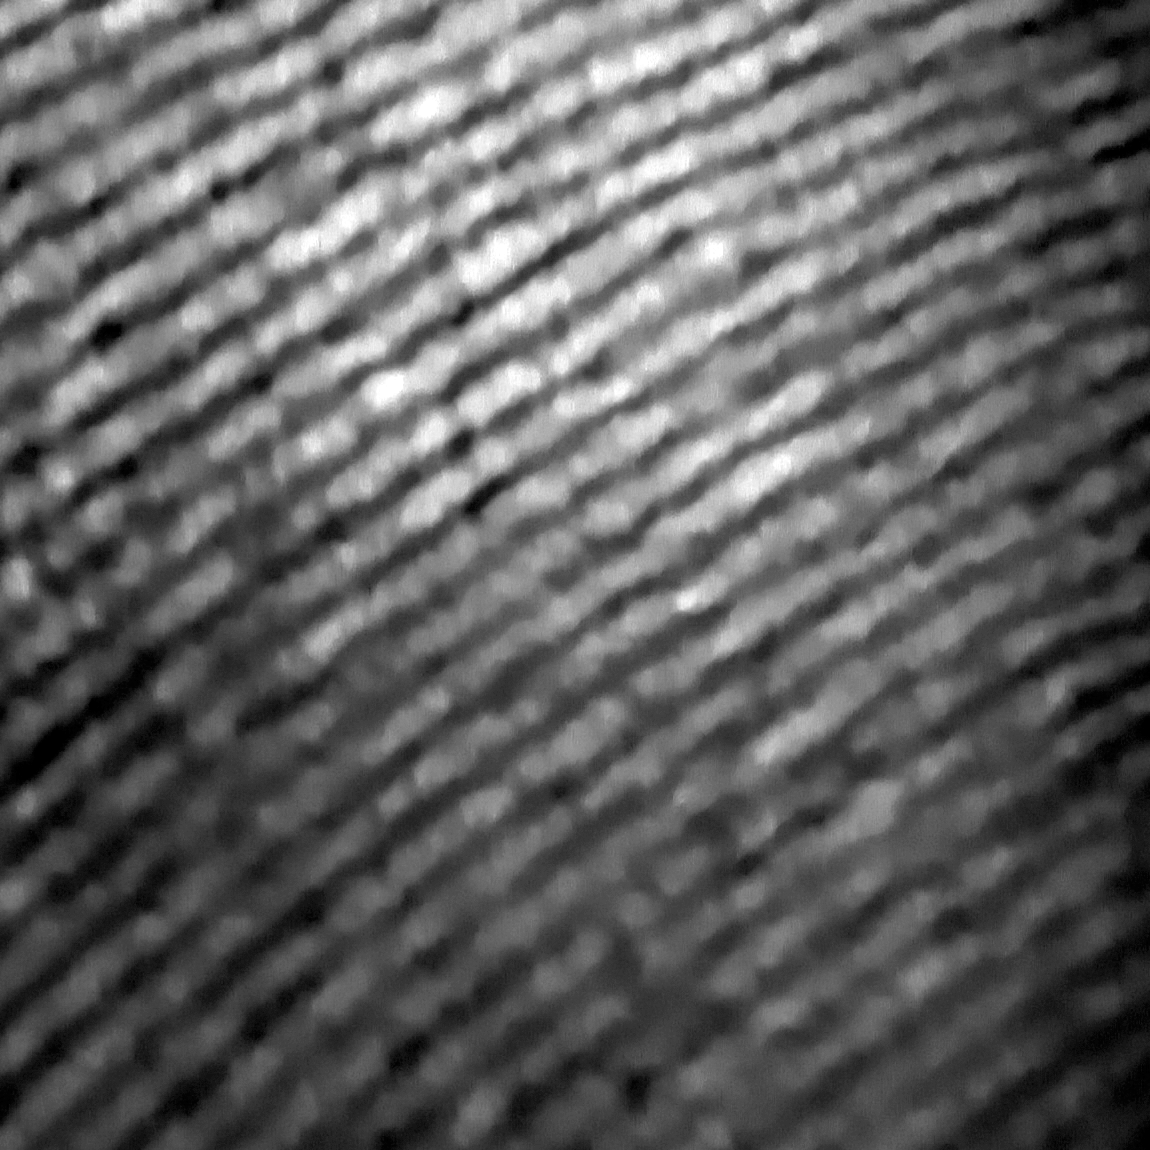
\includegraphics[width=0.25\textwidth]{images/straight_g.jpg}
				\caption{Straight line fringes}
			\end{figure}

			\item \textbf{Straight line fringes:} When $M_1$ and virtual image of $M_2$ intersect, straight line fringes are obtained around the point of intersection. The path difference along the line of intersection is zero and therefore, is same for all the wavelengths. The images are shown below.

		\end{itemize}

		% If the reflection of mirror M2 as seen through the beam splitter is exactly parallel to mirror M1, or simply when M2 is perpendicular to M1, then concentric circular fringes (fringes of equal inclination) will result. The fringes are formed depending on the inclination of the incident and reflected rays because the air film's width between the image and M1 is constant. The ray reflecting from the farther away mirror will travel an additional distance of 2d cos theta as shown in the figure below if the angle is, for example, $\theta$.


		% Therefore bands will be formed for the same inclination of light rays which corresponds to circular fringes. In the experiment we will deal with circular fringes for the two light source. As we change the path difference between the mirror from d $(2d = n\lambda)$, say $N$ fringes appear or disappear near the centre (that is inclination θ = 0. This implies: